\documentclass[10pt, a4paper, oneside]{article}
\usepackage[ngerman]{babel}

\usepackage{nccmath}

\usepackage{blindtext}
\usepackage{titlesec}
\usepackage{amsmath}
\usepackage[hidelinks]{hyperref}
\usepackage{parskip}
\usepackage{graphicx}
\usepackage{longtable}
\usepackage[shortlabels]{enumitem}
\usepackage{multirow}
\usepackage{nccmath}
\usepackage{rotating}
\usepackage{makecell}
\usepackage{multicol}
\usepackage{capt-of}
\usepackage{csquotes}
\usepackage{amsfonts}
\usepackage{caption}

\captionsetup[table]{position=bottom}

\titleformat{\section}
    {\normalfont\Large\bfseries}{}{0pt}{}

\let\oldsection\section
\renewcommand{\section}{
  \renewcommand{\theequation}{\thesection.\arabic{equation}}
  \oldsection}
\let\oldsubsection\subsection
\renewcommand{\subsection}{
  \renewcommand{\theequation}{\thesubsection.\arabic{equation}}
  \oldsubsection}

\makeatletter
\renewcommand{\maketitle}{
    \bgroup
    \centering
    \par\LARGE\@title  \\[20pt]
    \par\large\@author \\[10pt]
    \par\large\@date
    \par
    \egroup
}
\makeatother


\title{Mathematische Grundlagen\\[5pt]Lösungen zu den Aufgaben 1, 4, 6 und 11}
\author{Volodymyr But}
\date{WS24/25, FHS Trier}

% - - - - - - - - - - - - - - - - - - - - - - - - - - - - - - - - - - - - - - %

\begin{document}

\maketitle
\vspace{25px}

\section{Aufgabe 1}

Es seien $M := \{ -2, -\dfrac{1}{2}, 0,1, \pi, 5,7 \}$, $M_1 := \{-2, 0, 7\}$ und
$M_2 := \{ -\dfrac{1}{2}, 0, \pi, 5 \}$. Bestimmen Sie $$M_1 \cap M_2, M_1 \cup
M_2, M_1^{c(M)}, M_2^{c(M)}, M \setminus (M_1 \cup M_2)$$

\textbf{L"osung}.

\begin{enumerate}[(a)]
    \item $M_1 \cap M_2 = \{ x : x \in M_1$ und $x \in M_2 \} = \{ 0 \}$
    \item $M_1 \cup M_2 = \{ x : x \in M_1$ oder $x \in M_2 \} = \{ -2, 0, 7, -\dfrac{1}{2}, \pi, 5 \}$
    \item $M_1^{c(M)} = M \setminus M_1 = \{ x : x \in M$ und $x \notin M_1 \} = \{ -\dfrac{1}{2}, 1, \pi, 5 \}$
    \item $M_2^{c(M)} = M \setminus M_2 = \{ x : x \in M$ und $x \notin M_2 \} = \{ -2, 1, 7 \}$
    \item $M \setminus (M_1 \cup M_2) = \{ x : x \in M$ und $x \notin M_1$ und $x \notin M_2\} = \{1\}$
\end{enumerate}

\section{Aufgabe 4}

\begin{enumerate}[(a)]
    \item \begin{enumerate}[i)]
            \item Finden Sie ein \textbf{Gegenbeispiel}, das zeigt, dass
                folgende Aussage allgemein \textbf{nicht} gilt:\\
                Seien $M,M_1,M_2$ nicht-leere Mengen, sodass
                $$M_1 \subset M, \quad M_2 \subset M, \quad M_1 \cap M_2 = \emptyset$$
                Dann gilt auch
                $$M_1 \cup M_2 = M$$

                \textbf{L"osung}.
                Es seien $M := \{ 1, 2, 3, 4, 5, 6, 7, 8, 9 \}$, $M_1 := \{1,
                2, 3, 4\}$, $M_2 := \{6, 7, 8, 9\}$. Dann gilt:
                $$M_1 \subset M, \quad M_2 \subset M, \quad M_1 \cap M_2 = \emptyset$$
                Das bedeutet jedoch nicht, dass $M_1 \cup M_2 = M$, weil
                $$M_1 \cup M_2 = \{ 1, 2, 3, 4, 6, 7, 8, 9 \} \neq \{1, 2, 3, 4, \textbf{5}, 6, 7, 8, 9\} = M $$

            \item Geben Sie au{\ss}erdem ein Beispiel an, f"ur das die Aussage gilt.

                \textbf{L"osung}.
                Es seien $M := \{ 1, 2, 3, 4, 5, 6, 7, 8, 9 \}$, $M_1 := \{1,
                2, 3, 4\}$, $M_2 := \{\textbf{5}, 6, 7, 8, 9\}$. Dann gilt:
                $$M_1 \subset M, \quad M_2 \subset M, \quad M_1 \cap M_2 = \emptyset$$
                wie auch
                $$M_1 \cup M_2 = \{1, 2, 3, 4, \textbf{5}, 6, 7, 8, 9\} = M$$

            \item Verbinden Sie $M, M_1, M_2$ mithilfe der
                Komplement-Mengeoperation zu einer Formel, die f"ur den Fall
                aus ii) gilt.

                \textbf{Lösung}. Anhand des Beispiels aus ii) lässt sich feststellen, dass
                wenn $M,M_1,M_2$ nicht-leere Mengen sind, sodass
                $$M_1 \subset M, \quad M_2 \subset M, \quad M_1 \cap M_2 = \emptyset$$
                gilt die Aussage $M_1 \cup M_2 = M$ nur wenn
                $$M_1^{c(M)} = M_2 \quad\text{oder}\quad M_2^{c(M)} = M_1$$
          \end{enumerate}
    \item \begin{enumerate}[i)]
            \item  Schreiben Sie die folgende Menge in der beschreibenden Mengenschreibweise:
                \textit{Die Menge aller geordneter zwei-Tupel, wobei die erste
                Komponente eine ganze Zahl und die zweite Komponente eine n
                nat"urliche Zahl ungleich 0 ist und die beiden Zahlen sind
                teilerfremd}.

                \textbf{L"osung}.
                $$M = \{ (x_1, x_2) \in \mathbb{Z} \times \mathbb{N} : \text{ggT}(x_1, x_2) = 1\ \text{und}\ x_2 \neq 0 \}$$

            \item Welche allgemein bekannte Zahlen-Menge haben Sie gerade beschrieben?

                \textbf{L"osung}.
                Keine Ahnung :(
          \end{enumerate}
\end{enumerate}

\section{Aufgabe 6}

\begin{enumerate}[(a)]
    \item Skizzieren Sie die Menge $[-1, 3] \times \{-2,2,3\}$.

        \textbf{L"osung}.
        \begin{align*}
            M = [-1, 3] \times \{-2,2,3\} &= \{-1, 0, 1, 2, 3\} \times \{-2, 2, 3\} = \\
                                          &=
                    \begin{aligned}[t]
                        \{&(-1, -2), (-1, 2), (-1, 3), (0, -2), (0, 2),\\
                          &(0, 3), (1, -2), (1, 2), (1, 3), (2, -2), (2, 2),\\
                          &(2, 3), (3, -2), (3, 2), (3, 3)\}
                    \end{aligned}
        \end{align*}

        \begin{figure}[t]
            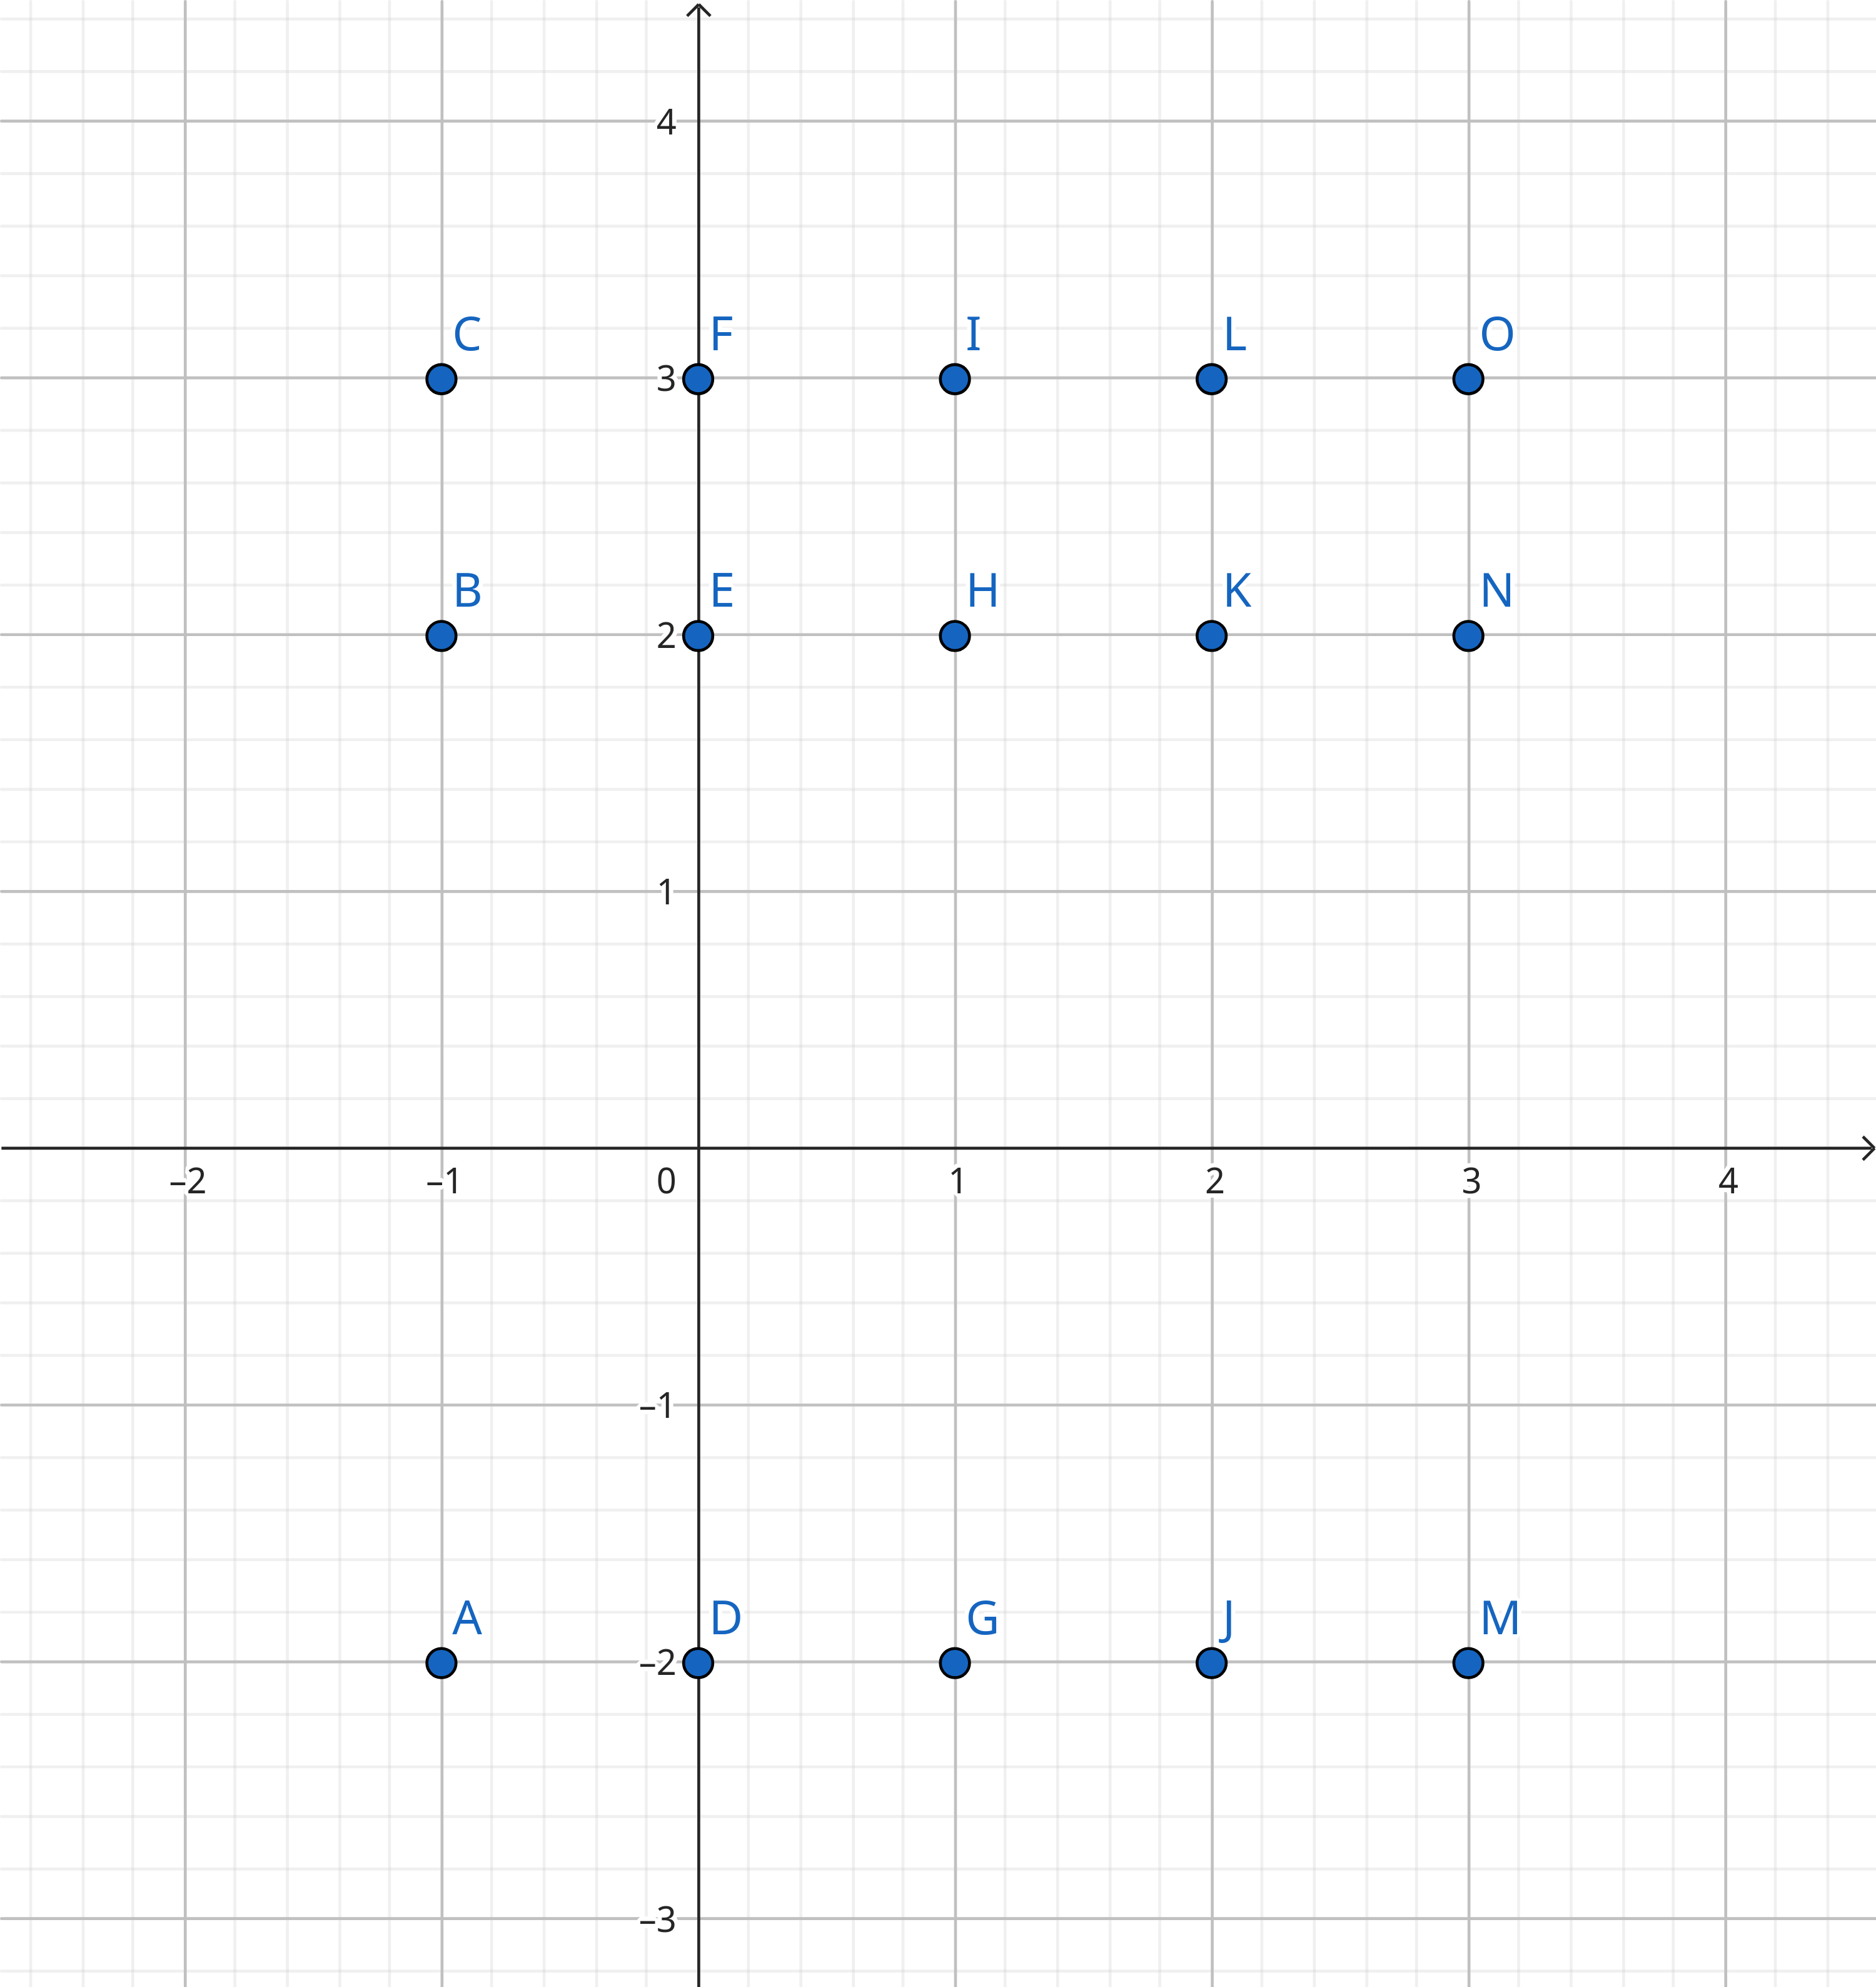
\includegraphics[width=1\textwidth]{./assets/skizze-1.png}
            \caption{$[-1,3] \times {-2,2,3}$}
        \end{figure}

    \pagebreak

    \item Schreiben Sie folgende Menge durch Aufz"ahlen all ihrer Elemente
        $(\mathbb{Z} \times \{-1, -2\}) \cap (\{3, 4\} \times \mathbb{Z})$.

        \textbf{L"osung}.
        \begin{align*}
            M &= (\mathbb{Z} \times \{-1, -2\}) \cap (\{3, 4\} \times \mathbb{Z}) =\\[5pt]
              &=
              \begin{aligned}[t]
                  \{(x_1, x_2) \text{ : }& x_1 \in \mathbb{Z} \text{, } x_2 \in \{-1, -2\} \text{ und}\\
                                         & x_1 \in \{3, 4\} \text{, } x_2 \in \mathbb{Z}\} =
              \end{aligned}\\
              &= \{(x_1, x_2) \text{ : } x_1 \in \{3, 4\} \text{, } x_2 \in \{-1, -2\}\} =\\[5pt]
              &= \{(3, -1), (3, -2), (4, -1), (4, -2)\}
        \end{align*}
\end{enumerate}

\pagebreak

\section{Aufgabe 11}

Pr"ufen Sie die folgenden Aussagen auf ihre G"ultigkeit, und beweisen Sie diese
bzw. widerlegen Sie diese durch ein Gegenbeispiel.

\begin{enumerate}[(a)]
    \item F"ur zwei Mengen $A,B$ mit $A \cap B = \emptyset$ gilt, es gibt keine
        Menge $C$ mit $C \subset A$ und $C \subset B$.

        \textbf{Beweis}.
        \begin{enumerate}[-]
            \item Wenn $A \cap B = \emptyset$ gilt, bedeutet das, dass $A$ und $B$ keine gemeinsamen Elemente haben.
            \item $C \subset A$ bedeutet, dass alle Elemente von $C$ auch in $A$ enthalten sind.
            \item $C \subset B$ bedeutet, dass alle Elemente von $C$ auch in $B$ enthalten sind.
        \end{enumerate}

        Da $A \cap B = \emptyset$, gibt es keine Elemente, die sowohl
        in $A$ als auch in $B$ liegen k"onnen. Daraus folgt, dass es
        keine Menge $C$ geben kann, die sowohl eine Teilmenge von $A$
        als auch von $B$ ist, au{\ss}er der leeren Menge  $C =
        \emptyset$.

        Die Aussage, dass es für zwei Mengen $A$ und $B$ mit $A \cap B = \emptyset$
        keine \underline{nicht-leere} Menge $C$ mit $C \subset A$ und $C
        \subset B$ geben kann, ist also \textbf{wahr}.


    \item F"ur Mengen $M_1, M_2, M_3, C$ gilt $C \subset (M_1 \cup M_2 \cup
        M_3)^c$ genau dann, wenn f"ur alle $j = 1, 2, 3$ $C \cap M_j = \emptyset$
        gilt.

        \textbf{Beweis}.

        \begin{fleqn}
            \begin{align*}
                     &C \subset M^{c(C)} \\
                \iff &C \subset C \setminus M \\
            \implies &\forall_{x \in C} : x \in (C \setminus M) \\
                \iff &\forall_{x \in C} : x \in \{y : y \in C, y \notin M \} \\
            \implies &\forall_{x \in C} : x \notin M \\
            \implies &C \cap M = \emptyset
        \end{align*}
        \end{fleqn}

        \begin{fleqn}
            \begin{align*}
                     &x \in (M_1 \cup M_2 \cup M_3)^c \\
                \iff &x \in (M_1^c \cap M_2^c \cap M_3^c) \\
                \iff &(x \in M_1^c) \land (x \in M_2^c) \land (x \in M_3^c)
            \end{align*}
        \end{fleqn}

        \begin{fleqn}
            \begin{align*}
                         &C \subset (M_1 \cup M_2 \cup M_3)^c \\
                \implies &\forall_{x \in C} : x \in (M_1 \cup M_2 \cup M_3)^c \\
                \implies &\forall_{x \in C} : (x \in M_1^c) \land (x \in M_2^c) \land (x \in M_3^c) \\
                \implies &(C \subset M_1^c) \land (C \subset M_2^c) \land (C \subset M_3^c) \\
                \implies &(C \subset M_1 = \emptyset) \land (C \subset M_2 = \emptyset) \land (C \subset M_3 = \emptyset)
            \end{align*}
        \end{fleqn}
        
\end{enumerate}

\end{document}
